\section{Behavior with Intact Observations}
\label{sec:behavior}

All behavioral statistics are computed from the dumped main-thread text of each validation
trajectory with one parser: assistant turns are split on the role marker, a think block is
empty when its content is whitespace, an observation is intact when a non-finish tool call is
followed by a complete \toolresp{} block, and branch, search, and open-page calls are counted
from their function tags. Branch-internal turns are folded away in the dumps and are not
counted; the trainer's own turn count, which includes them, is reported alongside.

\begin{table}[t]
\centering
\footnotesize
\begin{tabular}{lccccc}
\toprule
Checkpoint & Empty think & Branches/traj.\ & Overlong ($T{=}1.0$) & Main chars & Finish \\
\midrule
No-RL base & 51\% & 1.6 & 10\% & 38k & 89\% \\
\grpo{} 60 (59 steps) & 58\% & 2.5 & 18\% & 48k & 87\% \\
\foldgrpo{} 50 (46 steps) & 80\% & 4.4 & 32\% & 21k & 97\% \\
\bottomrule
\end{tabular}
\caption{Behavioral signatures at the last uncontaminated checkpoints. Empty-think share,
branch calls, main-thread length, and finish rate are computed over the 150 greedy
trajectories; the overlong (context blow-out) rate is the trainer's validation metric over the
600 temperature-1.0 trajectories.}
\label{tab:behavior}
\end{table}

\begin{figure}[t]
\centering
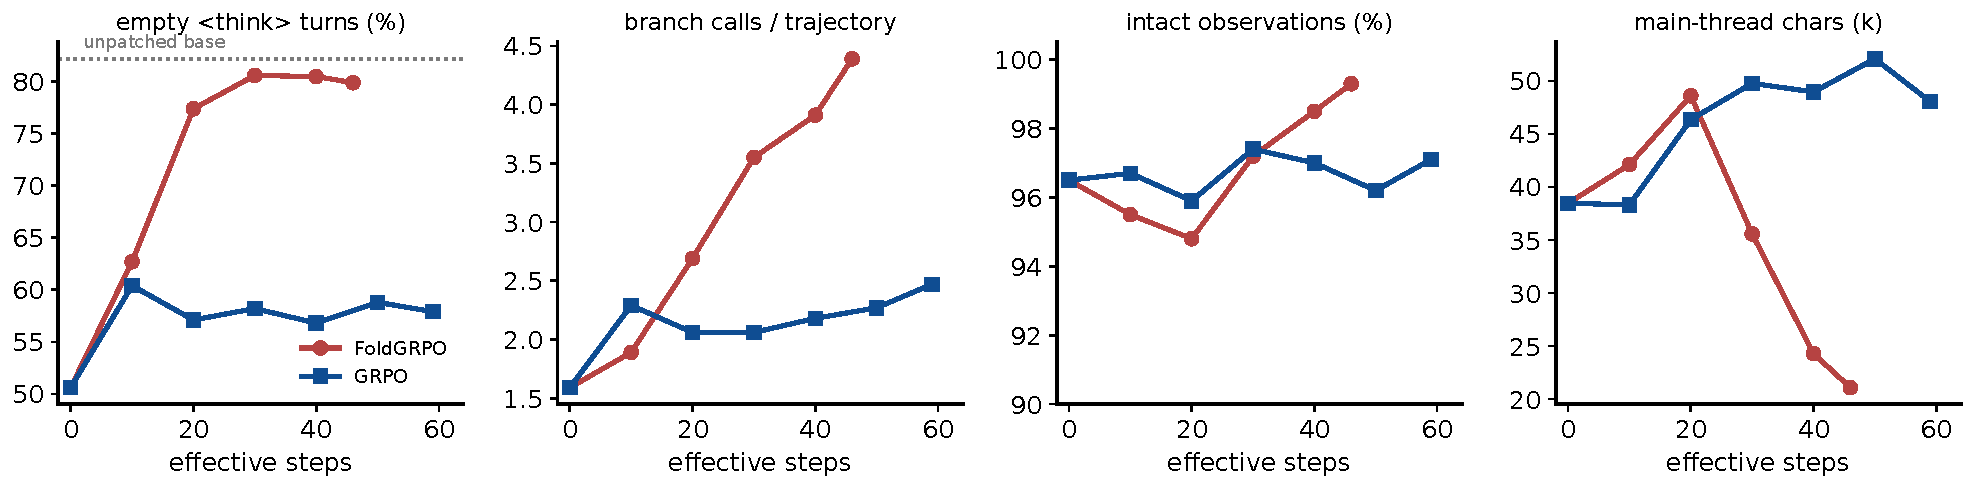
\includegraphics[width=\linewidth]{figures/fig3_behavior_vs_step.pdf}
\caption{Behavior per checkpoint from the greedy dumps (150 trajectories each; $x$ is
reward-bearing steps). Panels: share of assistant turns with an empty \think{} block (dotted
line: the unpatched base at 82\%); main-thread branch calls per trajectory; share of tool calls
followed by a complete observation; main-thread length in thousands of characters.}
\label{fig:behavior}
\end{figure}

\paragraph{Empty thinking rises under RL even with intact observations.} Observations stayed
95--99\% intact throughout training (\cref{fig:behavior}, third panel), so thinking no longer
costs the policy its observation. The empty-think share nevertheless climbed from 51\% at the
base to 77--81\% within 20 steps of \foldgrpo{} training and to 57--60\% within 10 steps of
\grpo{} training, and then plateaued (\cref{fig:behavior}, first panel). The earlier study had
attributed the trained policies' empty reasoning to adaptation to the corrupted format. That
explanation accounts for the base model's rate, which the fix halved, but not for the trained
policies' rate, which the fix did not change (\cref{fig:contrast}, middle). Under this reward
and at this scale, the outcome objective itself favors skipping visible reasoning, and the
process penalties of \foldgrpo{} push further in that direction.

\paragraph{Folding is learned; the blow-out advantage is not reproduced.} \foldgrpo{}'s
main-thread branch calls grew steadily to 4.4 per trajectory while \grpo{}'s plateaued at
about 2.3, and \foldgrpo{}'s main thread shrank to 21k characters against \grpo{}'s 48k
(\cref{tab:behavior}). The folding mechanism therefore emerges under the fixed code as it did
before. Its context-management benefit does not. At temperature 1.0 the \foldgrpo{} checkpoints
exhausted the 32k context in 24--32\% of trajectories against 13--18\% for \grpo{} and 10\%
for the base, the reverse of the earlier study's 0.04 versus 0.25. With intact observations
each turn carries more real content and \foldgrpo{}'s sub-trajectories are truncated more
often; the earlier six-fold blow-out advantage was in part an artifact of dropped observations
keeping contexts short. Finish rates were 87--97\% at the final checkpoints, and RL shifted
both arms from search-heavy toward branch-heavy main threads (search calls per trajectory
1.2 at the base, 0.3 for \foldgrpo{}, 1.3 for \grpo{}).
